%
% Complete documentation on the extended LaTeX markup used for Insight
% documentation is available in ``Documenting Insight'', which is part
% of the standard documentation for Insight.  It may be found online
% at:
%
%     http://www.itk.org/

\documentclass{InsightArticle}

\usepackage[dvips]{graphicx}

%%%%%%%%%%%%%%%%%%%%%%%%%%%%%%%%%%%%%%%%%%%%%%%%%%%%%%%%%%%%%%%%%%
%
%  hyperref should be the last package to be loaded.
%
%%%%%%%%%%%%%%%%%%%%%%%%%%%%%%%%%%%%%%%%%%%%%%%%%%%%%%%%%%%%%%%%%%
\usepackage[dvips,
bookmarks,
bookmarksopen,
backref,
colorlinks,linkcolor={blue},citecolor={blue},urlcolor={blue},
]{hyperref}


%  This is a template for Papers to the Insight Journal. 
%  It is comparable to a technical report format.

% The title should be descriptive enough for people to be able to find
% the relevant document. 
\title{Diffusion Tensor MRI Visualization in 3D Slicer 2.0}

% Increment the release number whenever significant changes are made.
% The author and/or editor can define 'significant' however they like.
\release{0.00}

% At minimum, give your name and an email address.  You can include a
% snail-mail address if you like.
\author{Lauren O'Donnell$^{1}$ and Raul San Jose Estepar$^{1}$}
\authoraddress{$^{1}$Brigham and Women's Hospital, Harvard Medical School, Boston MA USA}

\begin{document}


\ifpdf
\else
   %
   % Commands for including Graphics when using latex
   % 
   \DeclareGraphicsExtensions{.eps,.jpg,.gif,.tiff,.bmp,.png}
   \DeclareGraphicsRule{.jpg}{eps}{.jpg.bb}{`convert #1 eps:-}
   \DeclareGraphicsRule{.gif}{eps}{.gif.bb}{`convert #1 eps:-}
   \DeclareGraphicsRule{.tiff}{eps}{.tiff.bb}{`convert #1 eps:-}
   \DeclareGraphicsRule{.bmp}{eps}{.bmp.bb}{`convert #1 eps:-}
   \DeclareGraphicsRule{.png}{eps}{.png.bb}{`convert #1 eps:-}
\fi


\maketitle


\ifhtml
\chapter*{Front Matter\label{front}}
\fi


% The abstract should be a paragraph or two long, and describe the
% scope of the document.
\begin{abstract}
\noindent
This document describes our open source software for diffusion tensor
visualization and analysis.  The software is called DTMRI, after the
acronym DT-MRI, meaning diffusion tensor magnetic resonance imaging.
Its functionality includes tensor calculation from diffusion-weighted
images, tensor visualization using tractography and glyphs, and
measurement of scalar invariants such as anisotropy measures.  Other
features include clustering of tractography, selection of fibers based
on intersection with regions of interest, and conversion of fiber
trajectories to voxels for voxel-based analysis.  DTMRI is distributed
as a module in the 3D Slicer 2.0 open source medical image analysis
and visualization tool.

\end{abstract}

\tableofcontents

The goal of this paper is to give a high-level overview of the
functionality available in the DTMRI software.  We begin with a very
brief background section to familiarize the reader with the concept of
the diffusion tensor, then the remaining sections demonstrate the
capabilities of the software especially including the types of images
and 3D views that can be generated.  Finally we conclude with
instructions to obtain the software and additional references of
interest.


\section{Background on the Diffusion Tensor and Scalar Invariants}
Diffusion MRI measures the diffusion of water molecules in the brain.
The water molecules may diffuse faster in some directions than others,
depending on the cellular structure of the tissue. The diffusion
tensor is a mathematical model used to describe the amount of
diffusion in all directions, and from this model the principal, or
fastest, diffusion direction can be estimated. In white matter regions
where fibers do not cross, the direction of fastest diffusion
corresponds to the orientation of the white matter fiber tract.

The diffusion tensor is a $3 \times 3$ symmetric positive-definite
matrix that is proportional to the covariance matrix of water molecule
displacements during the imaging time.  Its major eigenvector
corresponds to the principal diffusion direction.  The tensor has
three eigenvalues ($formula ***** $) that quantify the diffusivity of water
in the principal diffusion direction and in two perpendicular
directions. From the tensor, various scalar invariants can be
calculated that describe the ``shape'' of the diffusion.  (The word
``scalar'' means a single number, as opposed to a vector or tensor.
The word ``invariant'' refers to the fact that these numbers are
invariant to rotation of the brain in the MRI machine, i.e. they do
not depend on the directions in which diffusion was measured, though
it is important to measure using enough directions).  By ``shape'' of
diffusion, we mean whether the diffusion is approximately equal in all
directions (spherical), in a plane or pancake shape (planar), or
mainly in one direction (linear).

For reference we include formulas for three common scalar invariants,
the trace, the fractional anisotropy (FA), and the linear measure
($c_L$). *******
%%%%%%%%%%%%%%%%%%%%%%%%%%%%%%%%%%%%%%%%%%%%%%%%%%%%%%%%%%
%
%  Example on how to insert an equation.
%  Never forget to put an equation in your paper. 
%  They make them look professional and impress the reviewers.
%
%%%%%%%%%%%%%%%%%%%%%%%%%%%%%%%%%%%%%%%%%%%%%%%%%%%%%%%%%%


\begin{equation}
\label{eqn:ShapeInfluenceTerm}
\xi \left(\psi^{*}(\mathbf{x}) - \psi(\mathbf{x})\right)
\end{equation}



\section{Diffusion Tensor Calculation}
The tensor is calculated as described in \cite{}.


\section{Diffusion Tensor Visualization}

\subsection{Glyphs}
A glyph is a 3D object which is oriented according to the tensor
eigenvector(s) and scaled by the tensor eigenvalue(s).  In addition,
color can be used with glyphs to indicate orientation or a scalar
invariant of the tensor.  Example images follow.

\subsection{Major Eigenvector Orientation as RGB Color}

In 3D Slicer, the coordinate system is RAS (right-anterior-superior)
and these directions are mapped to the red, green, and blue color
channels to produce images such as the following.


%%%%%%%%%%%%%%%%%%%%%%%%%%%%%%%%%%%%%%%%%%%%%%%%%%%%%%%%%%
%
%  Example on how to insert a figure
%
%%%%%%%%%%%%%%%%%%%%%%%%%%%%%%%%%%%%%%%%%%%%%%%%%%%%%%%%%%

\begin{figure}
\center
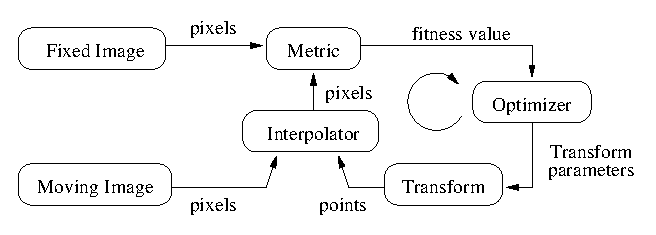
\includegraphics[width=0.8\textwidth]{RegistrationComponentsDiagram.eps}
\itkcaption[Registration Framework Components]{The basic components of the
registration framework are two input images, a transform, a metric, an
interpolator and an optimizer.}
\label{fig:RegistrationComponents}
\end{figure}



\section{Scalar Invariant Calculation}
The scalar invariants that can be calculated in DTMRI are listed in table \ref{table:Scalars}.

\section{Tractography}

\subsection{Tractography Clustering}


\section{Software Requirements}

You need to have the following software installed:

% The {itemize} environment uses a bullet for each \item.  If you want the 
% \item's numbered, use the {enumerate} environment instead.
\begin{itemize}
  \item  3D Slicer 2.x
\end{itemize}

Please refer to the following page for download information

\url{http://www.na-mic.org/Wiki/index.php/Slicer}


% The preceding sections will have been written in a gentler,
% introductory style.  You may also wish to include a reference
% section, documenting all the functions/exceptions/constants.
% Often, these will be placed in separate files and input like this:


%%%%%%%%%%%%%%%%%%%%%%%%%%%%%%%%%%%%%%%%%
%
%  Insert the bibliography using BibTeX
%
%%%%%%%%%%%%%%%%%%%%%%%%%%%%%%%%%%%%%%%%%

\bibliographystyle{plain}
\bibliography{Slicer2DTMRI}


\end{document}

